%%%%%%%%%%%%%%%%%%%%%%%%%%%%%%%%%%%%%%%%%%%%%%%%%%%%%%%%%%%%%%%%%%%%%%%%%%%%
%% Manuscript for IEEE Transactions on Cloud Computing.
%% Written from paper/focused/manuscript.tex (the skeleton) and its
%% OUTLINE.md. Every number comes from paper/focused/NUMBERS.md, which is
%% generated from results/*.json; scripts/check_tcc_numbers.py checks this.
%% Build: pdflatex -> bibtex -> pdflatex -> pdflatex
%%%%%%%%%%%%%%%%%%%%%%%%%%%%%%%%%%%%%%%%%%%%%%%%%%%%%%%%%%%%%%%%%%%%%%%%%%%%
\documentclass[10pt,journal,compsoc]{IEEEtran}

\usepackage{amsmath,amssymb}
\usepackage{graphicx}
\usepackage{booktabs}
\usepackage{algorithm}
\usepackage{algpseudocode}
\usepackage[nocompress]{cite}
\usepackage{url}
\makeatletter\let\inputtbl\@@input\makeatother
\providecommand{\checkmark}{\ensuremath{\surd}}

\newtheorem{theorem}{Theorem}
\newtheorem{lemma}{Lemma}
\newtheorem{definition}{Definition}
\newtheorem{remark}{Remark}

% Shared by the LaTeX build (manuscript.tex) and the Word build (build_docx.py).
\newcommand{\negl}{\mathsf{negl}}
\newcommand{\PPT}{\mathrm{PPT}}
\newcommand{\Real}{\mathbf{Real}}
\newcommand{\Ideal}{\mathbf{Ideal}}
\newcommand{\Leak}{\mathcal{L}}
\newcommand{\Sim}{\mathcal{S}}
\newcommand{\Adv}{\mathcal{A}}
\newcommand{\cind}{\approx_c}
\newcommand{\Gen}{\mathsf{Gen}}
\newcommand{\Eval}{\mathsf{Eval}}
\newcommand{\Enc}{\mathsf{Enc}}
\newcommand{\Dec}{\mathsf{Dec}}
\newcommand{\advPRF}{\mathrm{Adv}^{\mathrm{prf}}}
\newcommand{\advDPF}{\mathrm{Adv}^{\mathrm{dpf}}}
\newcommand{\advCPA}{\mathrm{Adv}^{\mathrm{cpa}}}
\newcommand{\bplus}{\boxplus}
\newcommand{\bdot}{\boxdot}


\begin{document}

\title{One-Round Verifiable Range Aggregation over Encrypted Data Replicated
across Non-Colluding Clouds}

\author{Md~Mazharul~Islam,
        Mubasshir~Ahmed,
        and~Md~Redowan~Zaman~Anik%
\IEEEcompsocitemizethanks{\IEEEcompsocthanksitem The authors are with the
Department of Electrical and Computer Engineering, North South University,
Plot 15, Block B, Bashundhara R/A, Dhaka 1229, Bangladesh.\protect\\
E-mail: mazharul.islam1@northsouth.edu (corresponding author),
mubasshir.ahmed@northsouth.edu, redowan.anik@northsouth.edu}}

\markboth{IEEE Transactions on Cloud Computing}%
{Islam \MakeLowercase{\textit{et al.}}: Verifiable Range Aggregation over Encrypted Multi-Cloud Data}

\IEEEtitleabstractindextext{%
\begin{abstract}
Internet of Things (IoT) deployments increasingly keep their data encrypted at
several cloud providers, while analysts need sums and counts over ranges of
time, place and sensor value. Existing systems for such queries either let the
clouds see which records a range selects, compute on unencrypted copies,
require an honest majority of servers that talk to each other, or cannot detect
a wrong answer from colluding clouds. We present a scheme for one-round range
aggregation over data that an owner encrypts once and replicates to $n$ clouds.
The owner stores encrypted summed-area tables, so that any $d$-dimensional box
is a signed sum of $2^d$ table entries. The analyst hides these entries in
distributed point function keys, and each cloud returns one ciphertext. A fresh
secret number carried inside a second set of keys lets the analyst detect a
wrong answer from up to $n-1$ colluding clouds without extra homomorphic work.
We evaluated the scheme on two public IoT datasets of about 400,000 records
each. A checked range query took 0.68--1.19\,s per cloud on one thread,
whatever the length of the range. It needed about 5\,kB of keys per cloud,
where a single-server homomorphic query needed 44\,MB. No tampered answer was accepted in 1,500 trials. The
range, the matching records, their number and the result stay hidden from any
$n-1$ colluding clouds.
\end{abstract}

\begin{IEEEkeywords}
Cloud security, homomorphic encryption, distributed point functions, range
queries, verifiable computation, Internet of Things.
\end{IEEEkeywords}}

\maketitle
\IEEEdisplaynontitleabstractindextext
\IEEEpeerreviewmaketitle

% ===========================================================================
\section{Introduction}
\label{sec:intro}

\IEEEPARstart{S}{ensor} networks in cities, hospitals and factories produce
large volumes of time-stamped readings~\cite{atzori2010internet}. The
organisation that collects the readings is often not the one that analyses
them. A city's air-quality office, for example, shares its measurements with
health agencies and researchers. The data are therefore stored in the cloud,
and many deployments keep copies at several providers for availability and to
avoid dependence on one vendor~\cite{petcu2013multicloud,grozev2014intercloud}.
Because the readings can be sensitive, the owner encrypts them before they
leave its control.

Analysts mostly ask for aggregates over ranges. A health agency may ask how
many hourly readings at one monitoring site fell into the five highest PM$_{2.5}$
bands during one month, and what their mean temperature was. This is a sum
over a box in three ordered dimensions: site, day and pollution band. We use
this question as a running example. Answering it over encrypted data raises
two problems. First, a cloud that learns which records a query touches learns
a great deal about the query and the data. Such access patterns are enough for
known attacks to recover plaintext~\cite{islam2012access,cash2015leakage,grubbs2017leakage}.
Second, the analyst has to trust that the cloud computed the answer correctly.

Single-server homomorphic encryption hides the query, but the encrypted query
must then be as large as the table it selects from. For one of the cubes in
our evaluation this is 44\,MB per query. Splitting the query among several
servers that do not collude avoids this cost: each server receives a short key
that reveals nothing on its own~\cite{chor1998private,gilboa2014distributed}.
Systems built this way, however, compute on unencrypted copies of the
data~\cite{splinter,hafiz2024private}, need an honest majority and
communication between servers~\cite{waldo,gupta2020obscure}, or support ranges
in one dimension only~\cite{splinter,gupta2020obscure}. None of them lets the
analyst detect a wrong answer from colluding servers at no extra cost.

We therefore seek a scheme with four properties:
\begin{itemize}
\item \textbf{(R1) Privacy against collusion.} Any $n-1$ of the $n$ clouds, pooling
what they see, learn neither the range nor which records match, how many
match, or the result.
\item \textbf{(R2) One round.} Each cloud receives one message and sends one reply.
Clouds never communicate with each other.
\item \textbf{(R3) Encrypted storage.} The owner encrypts the data once under its own
key. A cloud can be added or replaced by copying ciphertexts.
\item \textbf{(R4) Checked answers.} The analyst rejects a wrong answer from up to
$n-1$ deviating clouds.
\end{itemize}

Our scheme meets all four. Its main idea is to move the work of a range query
into precomputation. The owner places records in the cells of a data cube and
stores, for each cell, the running total of all cells below it. This is a
summed-area table~\cite{crow1984summed,ho1997range}. Any box is then the
signed sum of the table at its $2^d$ corners. The analyst turns each corner
into distributed point function (DPF) keys, one key per cloud. Each cloud
expands its keys over the whole table and multiplies the result into the
encrypted table. It returns a single ciphertext. The analyst adds the $n$
replies and decrypts the total of the box. Each cloud holds only its own share
of the selection, so no cloud ever sees which cells are selected.
Fig.~\ref{fig:system} shows the flow.

To check the answer, the analyst draws a fresh secret number $\delta_s$ for
each query. It sends a second set of keys in which every corner sign is
multiplied by $\delta_s$. Each cloud applies both key sets in the same
homomorphic operations, so its reply carries the answer $y$ and a check value.
The analyst accepts only if the check value equals $\delta_s y$. A coalition
that does not know $\delta_s$ cannot change the answer and keep this relation,
except with probability about $2^{-36}$ for our parameters.

Our contributions are as follows.
\begin{itemize}
\item A one-round protocol for $d$-dimensional range aggregation over
encrypted, replicated data. It applies the decomposition of a box into $2^d$
corners to an encrypted table instead of to the query, so the clouds never see
a record's coordinates. The work of a cloud and the size of its reply depend
neither on the range nor on the number of records.
\item A per-query check carried inside the DPF keys. We prove that a wrong
answer is accepted with probability at most $1/(p-1)$ plus the DPF advantage,
against any $n-1$ deviating clouds. We also show that the same check gives no
protection when a single server holds the whole query.
\item Security proofs, an implementation on OpenFHE and an evaluation on two
public IoT datasets. On the same machine we compare the scheme with two
alternatives: one key for every cell of the box, and a single server that
receives an encrypted query.
\end{itemize}

Each building block has a precursor. Boyle, Gilboa and Ishai decompose a
$d$-dimensional interval into $2^d$ anchored intervals for function secret
sharing~\cite[Cor.~3.4]{boyle2016function}. Summed-area tables come from
computer graphics and data cubes~\cite{crow1984summed,ho1997range}. A one-time
check key chosen by the client appears in PVODTE~\cite{li2026silent}, which
sends it to two servers under homomorphic secret sharing. What is new here is
how the parts fit together. The decomposition is applied to an encrypted table,
with dummy keys at the edges. The check key travels inside the DPF outputs, so
the check costs no homomorphic work and holds against $n-1$ colluding clouds.
To our knowledge, none of the systems in Table~\ref{tab:compare} provides
one-round, checked box aggregates over encrypted copies at this collusion
threshold.

The rest of the paper is organised as follows. Section~\ref{sec:related}
reviews related work. Section~\ref{sec:model} defines the model and the
building blocks. Section~\ref{sec:construction} presents the scheme and
Section~\ref{sec:security} its security. Sections~\ref{sec:setup}
and~\ref{sec:eval} describe the implementation and the evaluation.
Section~\ref{sec:discussion} discusses limitations, and
Section~\ref{sec:conclusion} concludes. Full proofs are in the supplemental
material.

% ===========================================================================
\section{Related Work}
\label{sec:related}

\emph{Queries split across servers.} Private information retrieval with
several non-colluding servers goes back to Chor et
al.~\cite{chor1998private}, and DPFs make the keys
short~\cite{gilboa2014distributed,boyle2015function,boyle2016function}.
Splinter~\cite{splinter} uses function secret sharing to answer sums, counts
and one-dimensional interval queries over public, unencrypted copies of the
data, and does not check results. Waldo~\cite{waldo} filters secret-shared time
series with three servers that interact and assumes an honest majority; in
return it is secure against malicious servers. Obscure~\cite{gupta2019obscure,gupta2020obscure}
answers counts, sums and top-$k$ queries over Shamir-shared data at servers
that do not communicate. A one-round predicate of length $l$ needs $2l+1$
servers, the adversary must not control a majority, and ranges are supported
in one dimension. Hafiz et al.~\cite{hafiz2024private} answer aggregate queries
in one round with information-theoretic retrieval over plaintext copies,
without range predicates. Single-server retrieval from lattices removes the
non-collusion assumption at a large query cost~\cite{angel2018pir,menon2022spiral},
and preprocessing reduces server work at the price of client
hints~\cite{corrigan2020private}.

\emph{Range aggregates at one server.} ARQ~\cite{espiritu2022arq} builds range
aggregates from structured encryption and leaks information that depends on the
query. HADES~\cite{liu2025hades} evaluates encrypted range predicates against a
single provider's plaintext database in one round, without result checks. It
reports that one-round homomorphic processing of a million encrypted records
takes more than fifteen hours. Timecrypt~\cite{timecrypt} and Zeph~\cite{zeph}
aggregate encrypted time series but reveal the queried interval. Prefix sums
for range sums are classical~\cite{ho1997range,crow1984summed}, and function
secret sharing supports intervals directly~\cite{boyle2016function}.

\emph{Checking answers.} Verifiable DPFs~\cite{decastro2022lightweight} and
access control for function secret sharing~\cite{pacl,ji2023finegrained}
protect the servers against a malicious client, not the client against
malicious servers. Verifiable homomorphic secret sharing~\cite{choudhuri2024vehss}
checks evaluation at the servers. PVODTE~\cite{li2026silent} has the client
send a one-time MAC key to two servers under homomorphic secret sharing,
secure against one malicious server. Our check uses the same kind of
information-theoretic MAC, a value $y$ together with $\delta_s y$ as in
SPDZ~\cite{damgard2012spdz}. It carries $\delta_s$ inside the DPF outputs
instead, needs no public-key operation and covers $n-1$ colluding clouds.
Table~\ref{tab:compare} summarises the closest systems.

\begin{table*}[t]
\caption{Systems closest to ours ($\checkmark$ yes, $\circ$ partly, $\times$ no).}
\label{tab:compare}
\centering
\footnotesize
\setlength{\tabcolsep}{4pt}
\begin{tabular}{@{}lccccc@{}}
\toprule
System & Data at the servers & Range aggregates & Colluding servers & Rounds between servers & Detects wrong answers \\
\midrule
Splinter~\cite{splinter} & plaintext copies & $\circ$ (1-D) & $n-1$ & none & $\times$ \\
Waldo~\cite{waldo} & secret-shared & $\checkmark$ & 1 of 3 & yes & $\checkmark$ \\
Obscure~\cite{gupta2020obscure} & Shamir-shared & $\circ$ (1-D) & minority & none & optional \\
Hafiz et al.~\cite{hafiz2024private} & plaintext copies & $\times$ & $n-1$ & none & $\circ$ \\
HADES~\cite{liu2025hades} & plaintext, one server & $\checkmark$ & n/a & n/a & $\times$ \\
ARQ~\cite{espiritu2022arq} & encrypted, one server & $\checkmark$ (with leakage) & n/a & n/a & $\times$ \\
\midrule
\textbf{This work} & encrypted copies & $\checkmark$ ($d$-D) & $n-1$ & none & $\checkmark$ \\
\bottomrule
\end{tabular}
\end{table*}

% ===========================================================================
\section{Model and Building Blocks}
\label{sec:model}

\subsection{Parties}
The scheme has three kinds of party (Fig.~\ref{fig:system}). The \emph{data
owner} collects the records, builds the encrypted tables and holds the secret
key $sk$ of the homomorphic scheme. Each of the $n$ \emph{clouds} stores a copy
of the encrypted tables and the public evaluation keys. A cloud never decrypts.
The \emph{analyst} is authorised by the owner, receives $sk$, sends queries and
combines the replies.

\begin{figure*}[t]
\centering
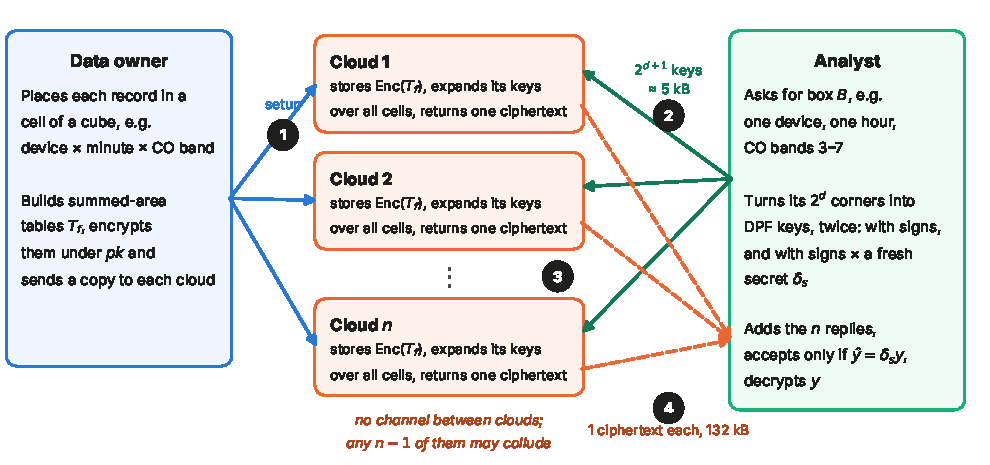
\includegraphics[width=0.92\textwidth]{figures/fig_system.pdf}
\caption{System overview. (1) The owner stores encrypted summed-area tables at
$n$ clouds. (2) The analyst sends each cloud its share of the query as DPF
keys. (3) Each cloud returns one ciphertext. (4) The analyst adds the replies,
checks them and decrypts.}
\label{fig:system}
\end{figure*}

\subsection{Data cubes and queries}
A \emph{data cube} has $d$ ordered attributes with $s_1,\dots,s_d$ values, and
so $M=\prod_k s_k$ cells. Every record $i$ lies in exactly one cell $c(i)$. In
the running example the attributes are site, day and PM$_{2.5}$ band. A
\emph{template} $f$ fixes what record $i$ contributes to an aggregate,
$w_f[i]\,m_i$: the constant $1$ for a count, the reading $m_i$ for a sum, its
square for a sum of squares. A \emph{range query} names a box
$B=\prod_k[\mathit{lo}_k,\mathit{hi}_k]$ and asks for
$\sum_{i:\,c(i)\in B}w_f[i]\,m_i$. Cubes and templates are registered by the
owner in advance; the boxes are chosen freely at query time. A mean is the
ratio of a sum and a count, and a variance follows from three templates.

\subsection{Threat model}
The adversary is static and runs in probabilistic polynomial time. It corrupts
a coalition of up to $t=n-1$ clouds. For privacy, the coalition follows the
protocol and pools everything its members see over adaptively chosen queries.
It must learn nothing beyond the leakage defined in Section~\ref{sec:security}:
not the box, not the matching records, not their number and not the result.
For correctness, the coalition may return any reply at all, and the analyst
must reject a wrong answer. The owner and the analyst are honest, and channels
are authenticated and encrypted. Side channels other than message sizes are
out of scope, as is collusion between the analyst and a cloud, since the
analyst can already decrypt.

\subsection{Building blocks}
\emph{Distributed point functions.} A point function $f_{\alpha,\beta}$ on
$[M]=\{0,\dots,M-1\}$ outputs $\beta\in\mathbb{Z}_p$ at $x=\alpha$ and $0$
elsewhere. An $n$-party DPF~\cite{gilboa2014distributed,boyle2015function,boyle2016function}
consists of $\Gen(1^\lambda,\alpha,\beta)$, which outputs keys
$\kappa_1,\dots,\kappa_n$, and $\Eval$, with
$\sum_j\Eval(\kappa_j,x)=f_{\alpha,\beta}(x)$ for every $x$. Any $n-1$ keys
reveal nothing about $\alpha$ or $\beta$, up to a distinguishing advantage
$\advDPF$. Two-party keys have $O(\lambda\log M)$ bits, and evaluating a key at
all $M$ points takes $O(M)$ pseudorandom-generator calls. For $n>2$ we use a
simple additive sharing in which $n-1$ clouds receive short seeds and one
receives an explicit vector.

\emph{Homomorphic encryption.} We use leveled BFV~\cite{fan2012somewhat} with
plaintext space $\mathbb{Z}_p$. It is IND-CPA secure with advantage $\advCPA$.
We write $\bplus$ for adding two ciphertexts and $\bdot$ for multiplying a
plaintext into a ciphertext. A BFV plaintext holds $\ell$ values in two rows
of $\ell/2$ slots, and rotations move values within a
row~\cite{halevi2014algorithms}. Table~\ref{tab:notation} lists the notation.

\begin{table}[t]
\caption{Notation.}
\label{tab:notation}
\centering
\small
\begin{tabular}{@{}ll@{}}
\toprule
Symbol & Meaning \\
\midrule
$n$ & number of clouds; up to $n-1$ may collude \\
$d$, $s_k$, $M$ & cube dimension, size of attribute $k$, cells \\
$C_f$, $T_f$ & cell totals and their summed-area table \\
$B$, $\kappa_\sigma(B)$ & box and its corner $\sigma\in\{0,1\}^d$ \\
$\beta_\sigma$ & sign of corner $\sigma$, or $0$ for a dummy \\
$e_j$ & cloud $j$'s keys evaluated at all cells and added \\
$\delta_s$ & per-query secret of the check \\
$p$, $\ell$ & plaintext modulus and number of BFV slots \\
\bottomrule
\end{tabular}
\end{table}

% ===========================================================================
\section{Construction}
\label{sec:construction}

\subsection{Computing on a shared selection}
\label{sec:oha}
The core operation lets the clouds sum selected table entries without any of
them knowing the selection. Suppose the analyst has split a selection vector
$e\in\mathbb{Z}_p^M$ into shares $e_1,\dots,e_n$ with $\sum_je_j=e$, and each
cloud holds the encrypted table $\Enc_{pk}(T_f)$. Cloud $j$ multiplies its own
share into the table and returns
\begin{equation}
\label{eq:contract}
\mathrm{ct}_j=\bplus_{x\in[M]} e_j[x]\bdot\Enc_{pk}(T_f[x]).
\end{equation}
The analyst adds the $n$ replies and decrypts. Since every operation is linear,
the result is $\sum_x e[x]\,T_f[x]$. Each cloud sees only its share, which on
its own is pseudorandom.

\begin{lemma}[One modulus]
\label{lem:compat}
If the DPF outputs and the BFV plaintexts live in the same ring $\mathbb{Z}_p$,
then $\bplus_j\mathrm{ct}_j$ decrypts to $\sum_x e[x]\,T_f[x]\bmod p$, except
with the probability that decryption fails.
\end{lemma}
\begin{IEEEproof}
Both $\bdot$ and $\bplus$ are homomorphisms of $\mathbb{Z}_p$-modules, so the
sum over the clouds commutes with decryption. Multiplying by a share, which is
a uniform element of $\mathbb{Z}_p$, scales the noise by up to $p$ without
consuming a level. The parameters of Section~\ref{sec:setup} absorb this, and
every query in Section~\ref{sec:eval} decrypted correctly.
\end{IEEEproof}

The condition is easy to violate in practice. DPF implementations often work
modulo $2^{64}$, while the homomorphic library uses its own prime. The
shares then add up correctly modulo $2^{64}$ but not modulo $p$, and every
answer is silently wrong. In our implementation the two use one modulus
object, so this error cannot be written.

\subsection{Range queries over summed-area tables}
\label{sec:range}
For a template $f$, the owner computes the total of every cell,
$C_f[c]=\sum_{i:\,c(i)=c}w_f[i]\,m_i$, and the summed-area table
\[
T_f[c]=\sum_{c'\le c}C_f[c'],
\]
where $c'\le c$ holds coordinate by coordinate. It lays the table out as a
column of $M$ entries and encrypts it. For a box $B$ and
$\sigma\in\{0,1\}^d$, let the corner $\kappa_\sigma(B)$ take
$\mathit{lo}_k-1$ on the attributes where $\sigma_k=1$ and $\mathit{hi}_k$
elsewhere. By inclusion and exclusion,
\begin{equation}
\label{eq:ie}
\sum_{c\in B}C_f[c]=\sum_{\sigma\in\{0,1\}^d}(-1)^{|\sigma|}\,T_f[\kappa_\sigma(B)].
\end{equation}
So the analyst needs $2^d$ table entries with signs $\pm1$. For each corner it
generates DPF keys for the point $\kappa_\sigma(B)$ with output
$\beta_\sigma=(-1)^{|\sigma|}\bmod p$. Each cloud evaluates its $2^d$ keys at
all $M$ cells and adds the results to obtain its share $e_j$, then applies
Eq.~\eqref{eq:contract}.

A corner can fall outside the cube. This happens when $\mathit{lo}_k=0$ on
some attribute, and such a corner contributes $0$. The analyst then sends a
\emph{dummy} key with output $0$ at a random cell. DPF keys hide the output as
well as the point, so a dummy key looks like any other. Every query to a cube
therefore carries exactly $2^d$ keys per cloud, and a box at the edge of the
cube cannot be told apart from one in the middle. Fig.~\ref{fig:rangeidea}
shows the two cases in two dimensions.

\begin{figure*}[t]
\centering
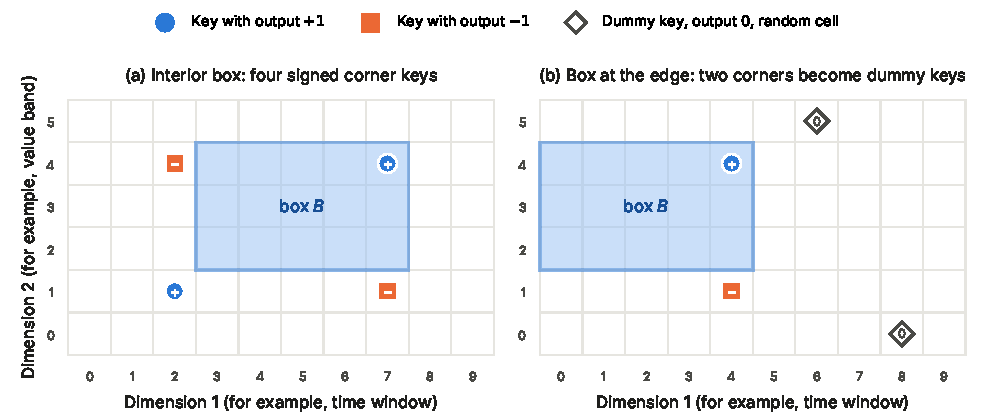
\includegraphics[width=0.85\textwidth]{figures/fig_range_idea.pdf}
\caption{A two-dimensional box as signed corners of the summed-area table. At
the edge of the cube, dummy keys keep the number of keys fixed.}
\label{fig:rangeidea}
\end{figure*}

Function secret sharing can also express an interval
directly~\cite{boyle2016function}. Applied to records, however, the servers
would need each record's coordinates in the clear, and here the coordinates
(which site, which day, which band) are the sensitive part. A dense encrypted
table over all cells hides them. The price is that cubes are registered in
advance and that the cost grows with the number of cells $M$, not with the
number of records.

\subsection{The per-query check}
\label{sec:check}
A BFV plaintext has two slot rows. The owner stores the table in row~0 and a
copy in row~1, so every reply can carry a check value next to the answer at no
extra size. The question is what the check value should be.

A natural choice is to store $\delta T_f$ in row~1 under a secret $\delta$
known to the analyst. This catches a cloud that changes only one row. It fails
against a cloud that changes both rows in the same way, for example by
multiplying its share by a constant before Eq.~\eqref{eq:contract}. The answer
and the check value then change in the ratio $\delta$, and the check passes.
Storing a different key $\delta_x$ for every cell catches changes at other
cells. It still misses a change at the queried cell itself, since there the
ratio is again the expected one. Section~\ref{sec:tampereval} measures both
failures.

Our check stores no key. For each query the analyst draws a fresh $\delta_s$
uniformly from $\mathbb{Z}_p^{*}$. Next to the $2^d$ keys with outputs
$\beta_\sigma$, it sends $2^d$ keys for the same points with outputs
$\delta_s\beta_\sigma$. Each cloud places the first evaluation in row~0 and the
second in row~1 of the same plaintexts. The homomorphic work is therefore
unchanged, and the combined reply decrypts to $y$ in row~0 and $\delta_s y$ in
row~1. The analyst accepts only if the two agree. Since $\delta_s$ is new for
every query and hidden in the keys, a deviating coalition cannot keep the
relation while changing $y$ (Theorem~\ref{thm:tamper}).

The check depends on the query being split, as the following remark shows.

\begin{remark}
\label{rem:single}
Suppose a single server holds the whole query, encrypted as $\Enc(e)$ in row~0
and $\Enc(\delta_s e)$ in row~1. It can replace $T_f$ by any table $T'_f$ in
both rows and return an encryption of
$(\langle e,T'_f\rangle,\delta_s\langle e,T'_f\rangle)$, which passes the
check. With two or more clouds, a coalition holds only shares of $e$ and of
$\delta_s e$, and the same change is caught.
\end{remark}

A test in our implementation runs both cases and observes the predicted
outcome.

\subsection{The protocol and its cost}
\label{sec:protocol}
Algorithm~\ref{alg:range} gives the protocol. Several templates, such as a
count and a sum, share one ciphertext: each occupies its own segment of the
two rows. The cloud sums each segment by rotations and, before sending, reduces
the ciphertext to one modulus tower, which halves its size without changing
the decrypted value.

\begin{algorithm}[t]
\caption{Checked range query on a registered cube.}
\label{alg:range}
\begin{algorithmic}[1]
\Statex \textbf{Setup} at the owner, once per cube and template $f$
\State $C_f[c]\gets\sum_{i:\,c(i)=c}w_f[i]\,m_i$; \ $T_f[c]\gets\sum_{c'\le c}C_f[c']$
\State put $T_f$ in row 0 and a copy in row 1; encrypt; send to every cloud
\Statex \textbf{Query} at the analyst, for box $B$
\State $\delta_s\gets\mathbb{Z}_p^{*}$ \Comment{fresh per query}
\ForAll{$\sigma\in\{0,1\}^d$}
  \State $c\gets\kappa_\sigma(B)$; \ $\beta\gets(-1)^{|\sigma|}$
  \If{$c$ is outside the cube} $c,\beta\gets$ random cell, $0$ \EndIf
  \State $(\kappa_{\sigma,j})_{j\le n}\gets\Gen(1^\lambda,c,\beta)$
  \State $(\hat\kappa_{\sigma,j})_{j\le n}\gets\Gen(1^\lambda,c,\delta_s\beta)$
\EndFor
\State send $\{\kappa_{\sigma,j},\hat\kappa_{\sigma,j}\}_\sigma$ to cloud $j$
\Statex \textbf{Answer} at cloud $j$
\State $e_j\gets\sum_\sigma\Eval(\kappa_{\sigma,j},\cdot)$; \ $\hat e_j\gets\sum_\sigma\Eval(\hat\kappa_{\sigma,j},\cdot)$
\State $\mathrm{ct}_j\gets$ Eq.~\eqref{eq:contract} with $e_j$ in row 0, $\hat e_j$ in row 1
\State sum each segment by rotations; compress; \Return $\mathrm{ct}_j$
\Statex \textbf{Combine} at the analyst
\State $(y,\hat y)\gets$ the two rows of $\Dec\big(sk,\bplus_j\mathrm{ct}_j\big)$
\If{$\hat y\neq\delta_s y$} reject \Else\ \Return $y$ \EndIf
\end{algorithmic}
\end{algorithm}

Per query and per cloud, the cost is $2^{d+1}$ evaluations of a key at all $M$
cells, $\lceil kM/(\ell/2)\rceil$ plaintext-ciphertext products for $k$
templates, and $\log_2(\ell/2k)$ rotations. The upload is $2^{d+1}$ keys of
$O(\lambda\log M)$ bits, and the reply is one ciphertext. None of these depends
on the box or on the number of records. The owner pays $O(M)$ per template at
setup.

% ===========================================================================
\section{Security}
\label{sec:security}

We first state what the clouds may learn. The \emph{setup leakage} is what a
cloud sees in its copy: $n$, $p$, $\ell$, the sizes $(s_1,\dots,s_d)$ of every
cube, and the number of templates and ciphertexts. The \emph{query leakage} is
which cube a query addresses and whether it carries the check keys. Together
these fix the number of keys. Nothing else is leaked: not the box, not the
matching records or their number, and not the result.

\begin{definition}[Security against $t$ colluding clouds]
\label{def:sec}
In the real experiment, the adversary chooses the data and a coalition $C$ of
at most $t$ clouds. It receives the coalition's stored state and then
adaptively issues $Q$ range queries. After each query it receives the
coalition's keys and the replies those clouds compute. In the ideal
experiment, a simulator produces the same view from the setup leakage and, for
each query, the query leakage. The scheme is secure if, for every efficient
adversary, an efficient simulator makes the two views indistinguishable except
with negligible probability.
\end{definition}

\begin{theorem}[Correctness]
\label{thm:correct}
Suppose $w_f[i]\,m_i\ge0$ for every record and the total of the cube,
$\sum_iw_f[i]\,m_i$, is below $p$. Then a query on box $B$ returns
$\sum_{i:\,c(i)\in B}w_f[i]\,m_i$, except with the probability that decryption
fails, and honest replies pass the check.
\end{theorem}
\begin{IEEEproof}[Proof sketch]
DPF correctness gives
$\sum_je_j=\sum_\sigma\beta_\sigma u_{\kappa_\sigma(B)}$, where $u_x$ is the
unit vector at $x$ and dummies have $\beta_\sigma=0$. By
Lemma~\ref{lem:compat} the combined reply decrypts to
$\sum_\sigma\beta_\sigma T_f[\kappa_\sigma(B)]\bmod p$, which
Eq.~\eqref{eq:ie} turns into the box total. That total lies in $[0,p)$, so the
reduction modulo $p$ loses nothing, although single terms are negative. Row~1
decrypts to $\delta_s$ times row~0. The full proof is in Supplemental
Section~S1.
\end{IEEEproof}

\begin{theorem}[Privacy against $n-1$ colluding clouds]
\label{thm:sec}
If $(\Gen,\Eval)$ is an $(n{-}1)$-private DPF and BFV is IND-CPA secure, the
scheme is secure against $t=n-1$ colluding clouds in the sense of
Definition~\ref{def:sec}, with distinguishing advantage at most
\[
Q\,2^{d_{\max}+1}\,\advDPF+m\,\advCPA ,
\]
where $d_{\max}$ is the largest cube dimension and $m$ the number of
ciphertexts the coalition stores.
\end{theorem}
\begin{IEEEproof}[Proof sketch]
A first sequence of hybrids replaces every DPF key the coalition receives by a
simulated key. This includes the dummy keys and the keys that carry
$\delta_s$, and is possible because DPF keys hide both point and output. A
second sequence replaces every stored ciphertext by an encryption of $0$. Each
reply is a deterministic function of a cloud's keys and stored state, so the
simulator recomputes it. As is standard for BFV, IND-CPA security is assumed to
hold given the rotation keys. The full proof is in Supplemental Section~S2.
\end{IEEEproof}

\begin{theorem}[Detection of wrong answers]
\label{thm:tamper}
Let up to $n-1$ clouds return arbitrary replies computed from their views,
with at least one cloud honest and $\delta_s$ known only to the analyst. The
analyst accepts an output $y'\neq y$, where $y$ is the correct answer, with
probability at most
\[
\frac{1}{p-1}+2^d\,\advDPF
\]
per query. Over $Q$ queries the bounds add.
\end{theorem}
\begin{IEEEproof}[Proof sketch]
Let $(r_0,r_1)$ be what the coalition's replies decrypt to in the two rows,
and $(y_C,\hat y_C)$ what they would have decrypted to if the coalition had
been honest. All four are functions of the coalition's view. The analyst
decrypts $y'=y-y_C+r_0$ and $\hat y'=\delta_sy-\hat y_C+r_1$, and accepts if
and only if $r_1-\hat y_C=\delta_s(y'-y)$. Replacing the coalition's keys that
carry $\delta_s$ by keys for an independent scalar changes the probability of
this event by at most $2^d\advDPF$. The view is then independent of
$\delta_s$. Since $y'-y\neq0$, at most one of the $p-1$ equally likely values
of $\delta_s$ satisfies the equation. The full proof is in Supplemental
Section~S3.
\end{IEEEproof}

The theorems have limits. A deviating cloud can always force a rejection, so
the scheme does not guarantee an answer. An analyst that reveals its
rejections can leak up to one bit about the data per query; retrying silently
through another set of clouds avoids this. Privacy is proved for clouds that
follow the protocol. Clouds never interact and receive only keys, however, so
a deviating coalition sees the same view and gains no information about the
query. The bound of Theorem~\ref{thm:tamper} is set by the plaintext modulus,
about $2^{-36}$ for our parameters. Running the check with $r$ independent
secrets lowers it to $(p-1)^{-r}+r\,2^d\advDPF$, at $r$ times the key
material; we implemented $r=1$.

One may ask whether secret-sharing the data could replace the encryption.
Under (R1)--(R3) it cannot. Answers over additive shares of the data contain
cross terms between one cloud's key share and another cloud's data share, and
no single cloud holds them. A scheme that avoided this without interaction
would yield single-server private information retrieval, which requires
public-key techniques~\cite{dicrescenzo2000single,kushilevitz1997replication}.
Supplemental Section~S4 gives the argument and the settings it does not cover,
such as an honest majority.

% ===========================================================================
\section{Implementation and Setup}
\label{sec:setup}

\emph{Implementation.} The reference implementation is written in Python and
calls the C++ kernels of OpenFHE~\cite{openfhe} for all homomorphic
operations. The two-party DPF is the tree construction of Boyle, Gilboa and
Ishai~\cite{boyle2016function} with fixed-key AES-128. BFV uses the plaintext
modulus $p=68{,}724{,}326{,}401$, a 37-bit prime with $p\equiv1\bmod2^{17}$,
ring dimension $8{,}192$ and multiplicative depth one, at the 128-bit security
level. The test suite compares range answers with brute force for $d\le3$ and
$n\le3$. It also contains failure controls: a flipped corner sign, for
instance, must give a wrong answer, and does. The code is not yet public and
is available from the corresponding author on reasonable request.

\emph{Datasets and cubes.} We use two public datasets. The Environmental
Sensor Telemetry dataset~\cite{stafford_2020_environmental} has 405,184
messages from three sensor arrays. Its cube is device (3) $\times$ minute
(11,523) $\times$ carbon-monoxide decile band (10), with $M=345{,}690$ cells.
The Beijing Multi-Site Air-Quality dataset~\cite{chen2019beijing,zhang2017cautionary}
has 420,370 hourly records with a temperature reading from twelve sites. Its
cube is site (12) $\times$ day (1,461) $\times$ PM$_{2.5}$ band (11: ten deciles
and one for missing readings), with $M=192{,}852$ cells. The templates are a
count and a sum of temperature in hundredths of a degree. Beijing temperatures
are shifted by $+50\,^\circ$C to keep every contribution non-negative, as
Theorem~\ref{thm:correct} requires. Each query fixes one device or site, a
window of $L$ minutes or days, and bands 3--7, as in the running example.

\emph{Machines and method.} The real-data runs used an AMD EPYC 7J13 server
with 32 virtual CPUs. The synthetic runs and the comparison with alternatives
used a cloud virtual machine with four virtual CPUs of an Intel Xeon at
2.1\,GHz. All runs use one thread, except where four worker processes are
named. Each reported time is the median of five runs, or of three for the
slowest alternatives. We do not compare times across the two machines. All
clouds ran on one host, so network time is not included; Section~\ref{sec:discussion}
estimates it. Every figure is drawn by a script directly from the result files.

% ===========================================================================
\section{Evaluation}
\label{sec:eval}

\subsection{Correctness}
\label{sec:correct}
Every range query in the experiments below decrypted to the box total computed
in plaintext. Each benchmark checks this before it records a time.

\subsection{Cost on real data}
\label{sec:realcost}
Fig.~\ref{fig:real} shows the time per cloud for windows from one minute or
day to the whole timeline. With the check, a query took 1,185.8--1,189.6\,ms
on the telemetry cube and 682.2--768.4\,ms on the Beijing cube. The time did
not grow with the window: a query over 11,523 minutes cost the same as a query
over one. This is expected, since every query evaluates the same number of
keys over the same table. A box at the corner of the cube, where most corners
become dummy keys, also cost the same, 1,192.6 and 758.9\,ms.

\begin{figure*}[t]
\centering
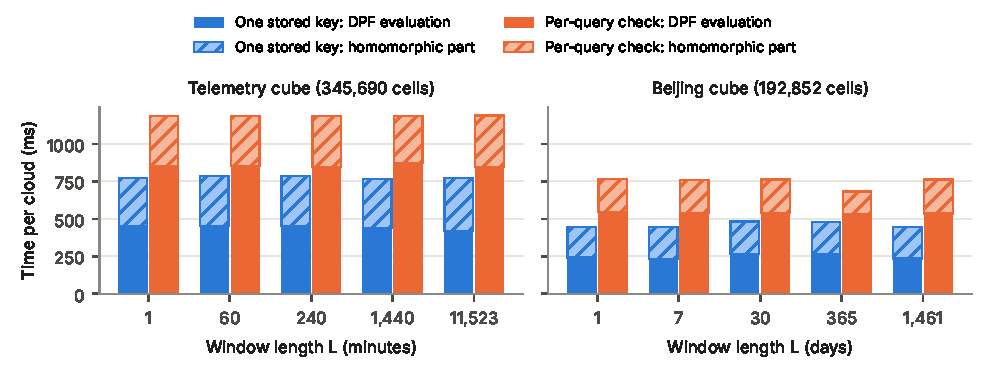
\includegraphics[width=0.92\textwidth]{figures/fig_range_real.pdf}
\caption{Time per cloud for range queries on the two real cubes, by window
length. Each bar is split into DPF evaluation and homomorphic work.}
\label{fig:real}
\end{figure*}

Evaluating the DPF keys took most of the time: 848.2--870.4\,ms on the
telemetry cube and 533.5--546.8\,ms on the Beijing cube. The check doubles the
number of keys but not the homomorphic work. With one stored check key instead,
the same queries took 767.8--788.3\,ms and 443.5--482.3\,ms. Every reply was
one ciphertext of 132,081 bytes. Each cloud received 5,520 or 5,248 bytes of
keys. The analyst spent 18.0--19.5\,ms generating the keys and
1.26--1.29\,ms combining, checking and decrypting the replies.

\subsection{Comparison with two alternatives}
\label{sec:baselines}
We answered the same queries in two other ways, on one machine and on a
synthetic cube with the dimensions of the telemetry cube
(Fig.~\ref{fig:baselines}). The first alternative, \emph{per-cell keys}, drops
the summed-area table. The clouds hold the encrypted cell totals, and the
analyst sends one point key for every cell of the box. It also takes one round
and uses the same homomorphic operation. The second alternative is a
\emph{single server}, which needs no assumption about collusion. The analyst
encrypts the signed corner vector, one ciphertext for each of the table's 169
ciphertexts, and the server multiplies the two ciphertext by ciphertext.

\begin{figure*}[t]
\centering
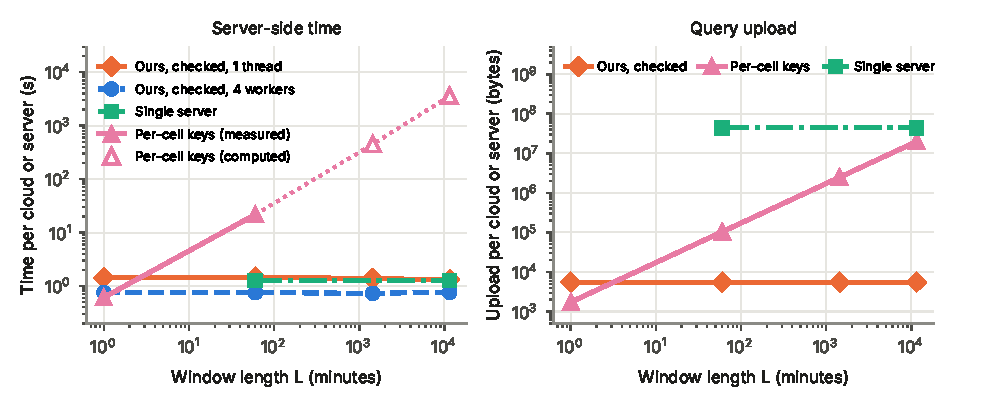
\includegraphics[width=0.92\textwidth]{figures/fig_range_baselines.pdf}
\caption{The same range query answered three ways on one machine: time at the
servers (left) and query upload (right). Open markers are computed, not
measured.}
\label{fig:baselines}
\end{figure*}

\emph{Without summed-area tables, the cost follows the box.} Per-cell keys
took 610.7\,ms for the 5 cells of a one-minute window and 21,710.8\,ms for the
300 cells of an hour. Our checked query took 1,301.6--1,457.0\,ms at every
length. We did not run the per-cell baseline for a day (7,200 cells) or the
whole timeline (57,615 cells). Extrapolating from the measured time per key,
62.2\,ms, gives about 7.5 and 60 minutes, with 2.5 and 19.9\,MB of keys per
cloud. This estimate is 13\% below the measured time for 300 cells, so it
understates the baseline. The number of keys also reveals the volume of the
box, unless every query is padded to the largest box allowed.

\emph{A single server needs a large query.} The single server took
1,269.8--1,274.5\,ms. One of our clouds with one stored key took
825.6--892.0\,ms, so two clouds together spend more server time than one
server. The split does not reduce total server work. It reduces the client's
work and traffic. The single-server query is 169 fresh ciphertexts, or
44,448,859 bytes, and encrypting it took 850.8--875.1\,ms at the client. Our
query is 5,520 bytes of keys per cloud, about 8,000 times smaller. The single
server also cannot use the check (Remark~\ref{rem:single}).

\emph{Key evaluation parallelises.} The $2^{d+1}$ key evaluations of a query
are independent. With four worker processes and the homomorphic work still on
one thread, a checked query took 731.4--765.3\,ms per cloud, and a query with
one stored key 505.3--547.4\,ms.

\subsection{Detecting wrong answers}
\label{sec:tampereval}
We injected five deviations by one of two clouds while the other stayed
honest. The deviating cloud (i) added a constant to the answer slot only,
(ii) added a uniform random vector to its share, (iii) multiplied its share by
a constant, (iv) added a constant to its share at a random cell, or (v) did the
same at a cell the query reads, as if it knew the query. Changes (ii)--(v)
affect both slot rows alike. Table~\ref{tab:tamper}
reports how often each change was detected and how often a wrong answer was
accepted.

\begin{table}[t]
\caption{Injected deviations by one of two clouds: detected / accepted with a
wrong answer.}
\label{tab:tamper}
\centering
\footnotesize
\setlength{\tabcolsep}{2.5pt}
\begin{tabular}{@{}lccccc@{}}
\toprule
Check & (i) & (ii) & (iii) & (iv) & (v) \\
\midrule
\inputtbl tamper_range.tex
\bottomrule
\end{tabular}
\end{table}

One stored key caught only the change to a single slot. Every change to both
rows was accepted with a wrong answer. Per-cell stored keys caught every
change except the one at a cell the query reads, which passed in all 200
trials. The
per-query check detected all five deviations in all 1,000 trials on the
synthetic cube and in all 500 trials on the two real cubes. These trials test
the implementation; they do not measure the bound of
Theorem~\ref{thm:tamper}.

\subsection{Layouts and cube size}
\label{sec:layouts}
Fig.~\ref{fig:layouts} (left) compares the three check layouts on the
synthetic cube. Per-cell stored keys need one table copy per corner and took
3.24--3.44\,s per cloud. The per-query check took 1.40--1.53\,s, and one stored
key 0.78--0.91\,s. The per-query check therefore costs less than half of the
per-cell layout and catches the attack that the per-cell layout misses.
Fig.~\ref{fig:layouts} (right) varies the number of cells for a
two-dimensional cube. A query took 34.7, 129.3 and 1,356.0\,ms for 10,000,
99,856 and 1,000,000 cells. The cost grows linearly with the cube, so the
number of cells, not the number of records or the length of the range, is what
a deployment must provision for.

\begin{figure*}[t]
\centering
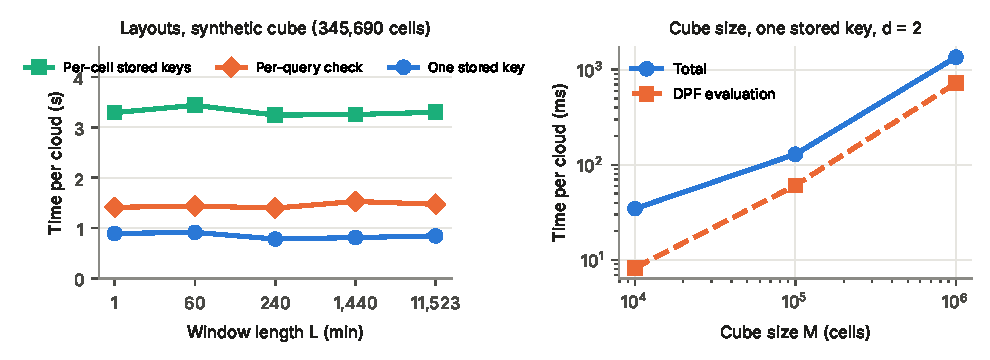
\includegraphics[width=0.92\textwidth]{figures/fig_range_layouts.pdf}
\caption{Time per cloud by check layout and window length (left) and by cube
size (right), on synthetic cubes.}
\label{fig:layouts}
\end{figure*}

% ===========================================================================
\section{Discussion and Limitations}
\label{sec:discussion}

\emph{What the split buys.} Against a single server that holds the same
encrypted table, non-colluding clouds do not save server time. They shrink the
query from tens of megabytes to kilobytes, remove the client's encryption
work, and make the check sound, because no cloud holds the whole query. The
design therefore suits analysts behind thin or metered links who need checked
answers. A client that can afford a 44\,MB query per range and needs no check
is served as well by one server.

\emph{Wide-area cost.} Each query is one message to each cloud and one reply,
with no exchange between clouds. A wide-area deployment therefore adds one
round trip and the transfer of about 5.5\,kB up and 132\,kB down per cloud.
At a round-trip time of 100\,ms and 20\,Mbit/s this is about 0.16\,s. This
figure is computed from the measured message sizes; we did not measure a
deployment across regions.

\emph{Limitations.} Our measurements come from a Python driver over C++
kernels, so a native implementation should be faster. Cubes and templates are
fixed at setup, every contribution must be non-negative, and the total of a
cube must stay below $p$. Privacy is proved for clouds that follow the
protocol; against deviating clouds we guarantee detection, not an answer. For
$n>2$ our keys are not succinct, since one cloud receives an explicit vector.

% ===========================================================================
\section{Conclusion}
\label{sec:conclusion}
Analysts of IoT data need range aggregates over data that is encrypted and
stored at several clouds. We showed how to answer such queries in one round
while hiding the range, the matching records, their number and the result from
any $n-1$ colluding clouds. Encrypted summed-area tables turn every box into
$2^d$ point keys, and a secret drawn for each query lets the analyst detect
wrong answers at no extra homomorphic cost. On two real IoT datasets a checked
query took about one second per cloud on one thread, independent of the
range, with kilobytes of upload. Future work includes a native
implementation, a deployment across cloud regions, succinct keys for more than
two clouds, and support for several data owners.

% ===========================================================================
\ifCLASSOPTIONcompsoc
  \section*{Acknowledgments}
\else
  \section*{Acknowledgment}
\fi
This research did not receive any specific grant. The authors declare no
competing interests. In line with IEEE policy on AI-generated content, we
disclose the following. Claude (Anthropic) drafted the text of all sections of
this article, including the statements and proofs of the theorems, from the
authors' earlier manuscripts. It also wrote the reference implementation, its
tests, the benchmark scripts and the scripts that draw every figure, ran the
synthetic-data experiments on a cloud virtual machine, and searched and
compared the literature. ChatGPT (OpenAI) and Gemini (Google) were used to edit
and review earlier drafts. The authors ran the real-data experiments, reviewed and edited
every section, checked the results against the implementation, and take full
responsibility for the content.
% AUTHORS: the last sentence must be true when you submit. Read every
% section and the proofs before uploading.

\bibliographystyle{IEEEtran}
\bibliography{references}

\end{document}
